\section{Vergleich der Algorithmen}
\subsection{Euklid}
\subsection{Dijkstra}
\subsection{Fast Marching}




\section{Einfluss der Zellgröße auf die Abstandsberechnung}
Bei der Berechnung der Abstände hat die Wahl der Zellgröße je nach Algorithmus einen entscheidenden Einfluss auf die Ergebnisse der Simulation. Die Zellgröße gibt nicht nur die minimale Schrittweite vor, sondern hat auch Einfluss auf die Genauigkeit der Nutzenberechnungen. Um einen Vergleich darzustellen wurde ein Quadratisches Feld angelegt. Die Zellgröße des Feldes sowie die Anzahl der Felder wurden so variiert, dass die Entfernung von der rechten unteren Ecke zur linken oberen Ecke (am weitesten entfernter Punkt) immer den gleichen Abstand hat. Es wird also die Diagonale des Rechtecks berechnet. Die Abbildung \ref{fig_euklid_fast_marching_2m_cellsize} Zeigt den Vergleich beider Algorithmen bei der der Abstandsberechnung. Üblicherweise wird die Rabskala so gewählt um alle Werte vom kleinsten Abstand zum weitesten Punkt abzubilden. Um den Vergleich an dieser Stelle deutlich zu machen, wurde für beide Bilder die selbe Farbskala verwendet. Mit Bloßem Auge ist die Differenz nur schwer zu erkennen. Es ist jedoch sichtbar, dass das Feld, welches mit dem Euklid algorithmus berechnet wurde, einen deutlicheren Bogen aufweist. 

Eine Möglichkeit die Unterschiede zu visualisieren ist es, die Bilder mittels einer Differenzbildung der Beiden Bilder. Dafür wird ein Bild als Basis hergenommen und das zweite Bild als eine Ebene darber eingefügt. Die Farben der zweiten Ebene werden von der ersten Ebene Subtrahiert. Gleichen sich die Farben beider Ebenen, so ist das Ergebnis schwarz. Dieser Vergleich macht nur Sinn, wenn für beide Darstellungen die selbe Farbskala verwendet wurde, also die Entfernungen mit dem gleichen Farbcode codiert wurden. Die Abbildung \ref{fig_fast_marching_euclid_difference} zeigt die Differenzmenge der in Abildung \ref{fig_euklid_fast_marching_2m_cellsize} dargestellten Karten.
An diesem Bild ist deutlich zu erkennen, dass die Zellen, welche sich nur in X und nur in Y Richtung vom Ziel entfernen schwarz sind.  Es gibt also keinen Unterschied zwischen dem Euklidischen Abstand und dem Abstand welcher mittels Fast Marching berechnet wurde, bei einer Betrachtung der Zellen nur in X oder nur in Y Richtung. Entfernt man sich schräg vom Ziel (Also X und Y Anteil gleichzeitig), sieht man deutlich Differenzen der beiden Algorithmen.


Die Tabelle \ref{tab_euklid_fm_vergleich} zeigt die Ergebnisse dieses Experiments. Die Cellsize gibt dabei die Kantenlänge einer quadratischen Zelle an. Wichtig ist der Wert „Distance in X and Y“, welcher besagt, dass das Ziel in X und in Y Richtung immer jeweils 14 Zellen entfernt ist.
Nach der Formel wurde der Abstand von Ziel zum am weitesten entfernten Punkt berechnet:

$$a = \sqrt[]{x^2 +y^2} = \sqrt[]{(14\ m) ^2 +(14\ m) ^2} = 19,799\ m$$ 

Wie in der Tabelle zu sehen ist, berechnet der Euklid Algorithmus den Abstand sehr präzise. Da der Euklid Algorithmus kein „Gedächtnis“ hat also ohne Einfluss vorheriger Zellen berechnet und die oben genannte Formel anwendet ist der Algorithmus gut geeignet um die exakte Entfernung zu berechnen. Interessant in der Tabelle ist vor allem die Abweichung von 1,45 m, welche beim Fast Marching Algorithmus entsteht. Diese Abweichung entspricht einem Fehler von von 7,3 \% bezogen auf die tatsächliche Entfernung. Verringert man die Zellgröße, so konvergiert der Fast Marching Algorithmus gegen den euklidischen Abstand und der Fehler gegen 0. Die prozentualen Fehler in Abhängigkeit der Zellgröße sind in Abbildung \ref{fig_fast_marching_error_cellsize} dargestellt. 

\section{Einfluss der Zellgröße auf die maximale Dichte}
Darüber hinaus hat die Zellgröße direkten Einfluss auf die Dichte [$\frac{Personen}{m^2}$] in einem Feld. Würde man die Zellgröße von $2\ m^2$ wählen, erhielte man eine maximale Dichte von 0,5 $\frac{1}{m^2}$. Es ist darauf zu achten, dass die Zellgröße angemessen gewählt wird. Bei weiteren Versuchen wurde stets eine Zellbreite von 0,4 bis 0,5 m verwendet, sofern nichts anderes angegeben.



\begin{figure}
\centering
\begin{minipage}{.44\textwidth}
\centering
  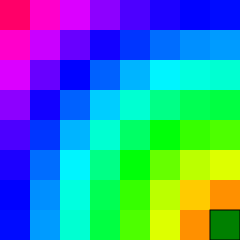
\includegraphics[width=0.9\linewidth]{abbildungen/vergleich_euklid_fast_marching/eEuclid_2m.png}
\end{minipage}%
\begin{minipage}{.44\textwidth}
\centering
  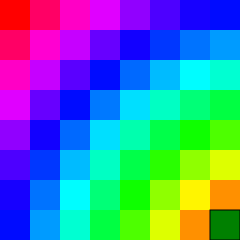
\includegraphics[width=0.9\linewidth]{abbildungen/vergleich_euklid_fast_marching/eFastMarching_2m.png}
\end{minipage}
\begin{minipage}{.1\textwidth}
\centering
  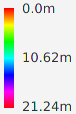
\includegraphics[width=\linewidth]{abbildungen/vergleich_euklid_fast_marching/farbskala.png}
\end{minipage}
\caption{Berechnung der Abstände mittels Euklid (links) und Fast Marching (rechts) an einem Feld mit einer Zellbreite von 2\ m. Dunkelgrün: Ziel, Rot: am weitesten entfernter Punkt im Feld}
\label{fig_euklid_fast_marching_2m_cellsize}
\end{figure}



\begin{figure}[ht]
	\centering
  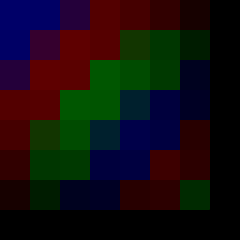
\includegraphics[width=0.4\textwidth]{abbildungen/vergleich_euklid_fast_marching/differenz_euklid_fast_marching.png}
	\caption{Differenzbildung der beiden Karten Euklid und Fast Marching}
	\label{fig_fast_marching_euclid_difference}
\end{figure}



\begin{table}[htbp]
\begin{tabular}{|l|r|r|r|r|r|r|r|}
\hline
Cellsize [m] & 2 & 1 & 0,5 & 0,25 & 0,125 & 0,0625 & 0,03125 \\ \hline
Cells in X and Y & 7 & 14 & 28 & 56 & 112 & 224 & 448 \\ \hline
Distance in  & & &  & &  & &\\ X and Y [m] & \textbf{14} & \textbf{14} & \textbf{14} & \textbf{14} & \textbf{14} & \textbf{14} & \textbf{14} \\ \hline
Tatsächliche & & &  & &  & &\\Entfernung [m] & 19,799 & 19,799 & 19,799 & 19,799 & 19,799 & 19,799 & 19,799 \\ \hline
Euklid [m] & 19,799 & 19,799 & 19,799 & 19,799 & 19,799 & 19,799 & 19,799 \\ \hline
Fast  & & &  & &  & &\\ Marching [m] & \textbf{21,245} & \textbf{20,717} & \textbf{20,363} & \textbf{20,137} & \textbf{19,997} & \textbf{19,913} & \textbf{19,863} \\ \hline
Diff [m] & 1,45 & 0,92 & 0,5645 & 0,3380 & 0,1979 & 0,1138 & 0,0644 \\ \hline
 & \multicolumn{1}{l|}{} & \multicolumn{1}{l|}{} & \multicolumn{1}{l|}{} & \multicolumn{1}{l|}{} & \multicolumn{1}{l|}{} & \multicolumn{1}{l|}{} & \multicolumn{1}{l|}{} \\ \hline
Error [\%]  & & &  & &  & &\\ diff/distance & \textbf{7,30} & \textbf{4,64} & \textbf{2,85} & \textbf{1,71} & \textbf{1,00} & \textbf{0,57} & \textbf{0,33} \\ \hline
\end{tabular}
\caption{Vergleich der Algorithmen Fast Marching und Euklid. Cellsize ist die Kantenlänge einer quadratischen Zelle in m (Zellbreite)}
\label{tab_euklid_fm_vergleich}
\end{table}


\begin{figure}[ht]
	\centering
  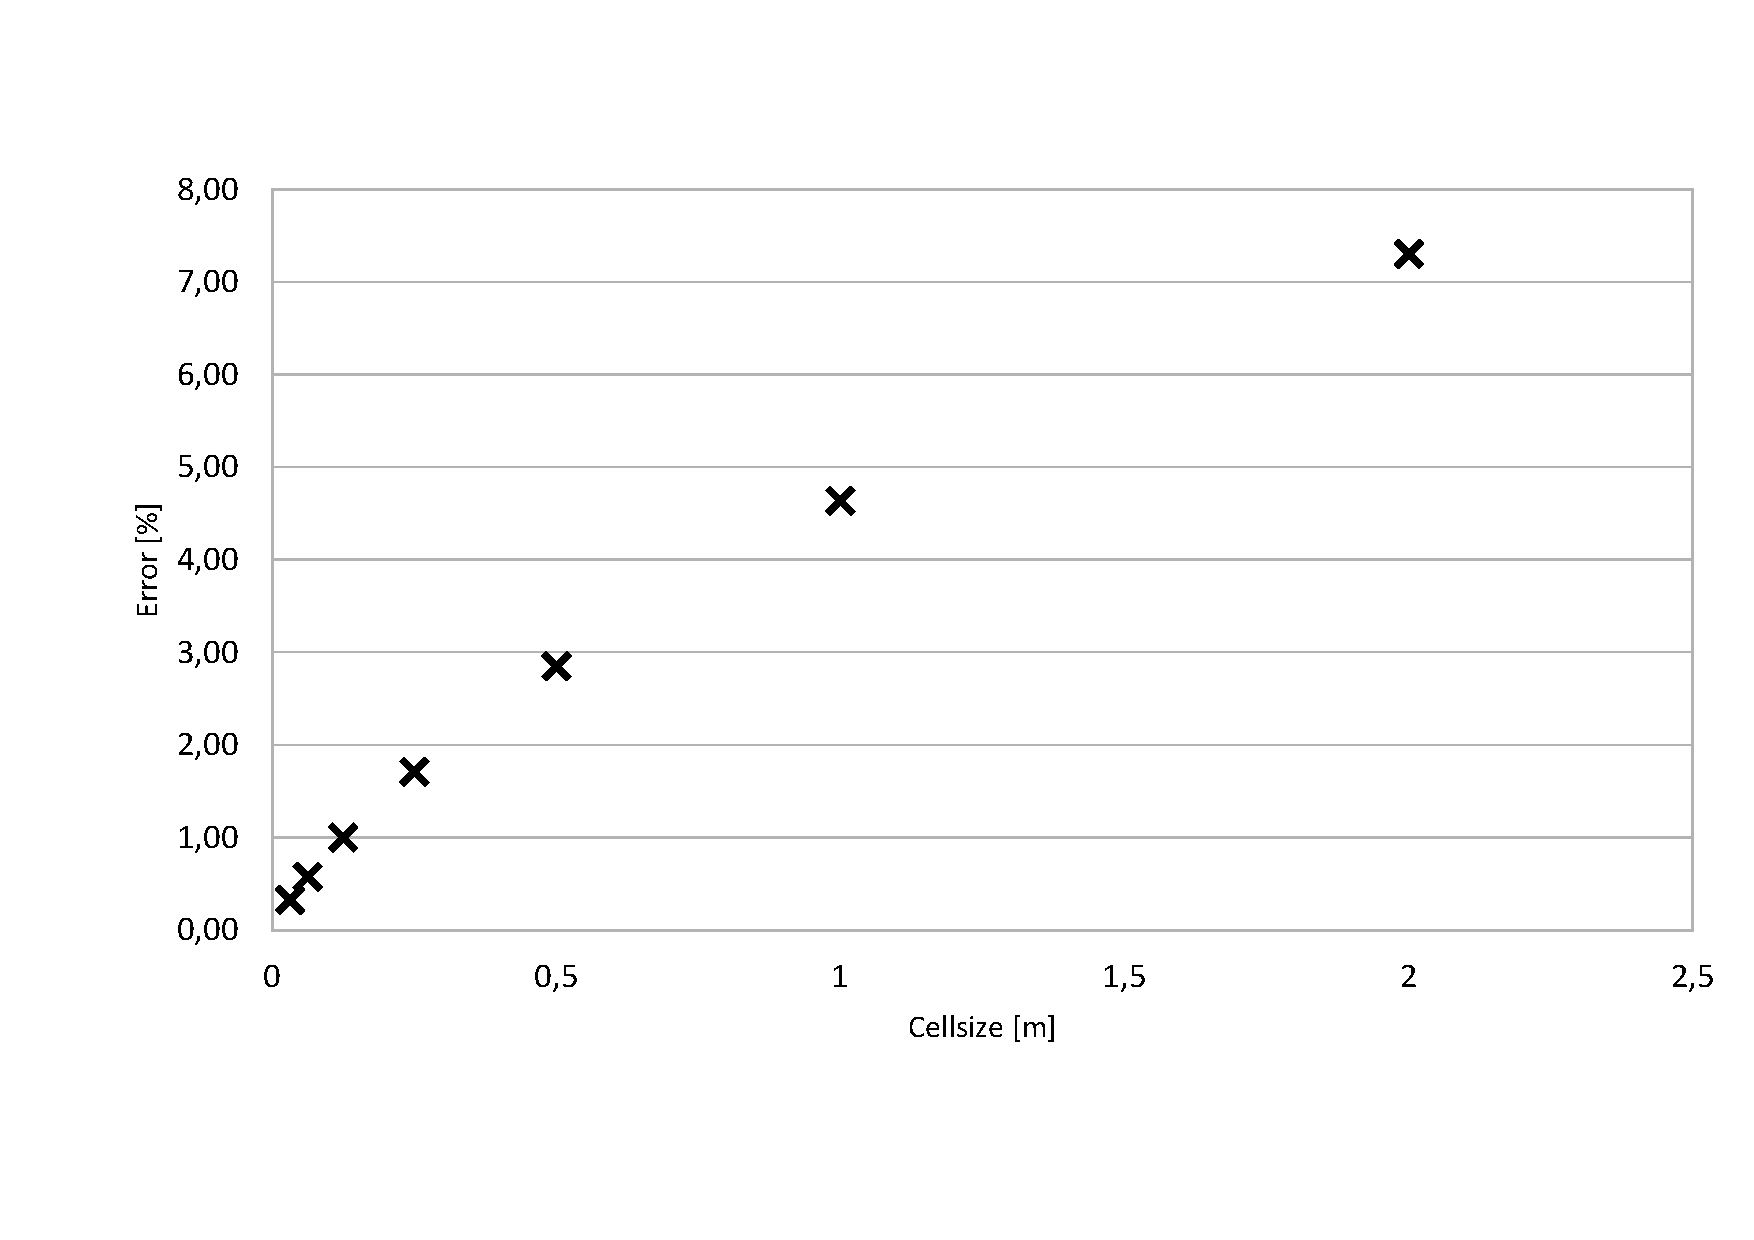
\includegraphics[width=\textwidth]{abbildungen/vergleich_euklid_fast_marching/EuklidFastMarchingError.pdf}
	\caption{Prozentualer Fehler des Fast Marching Algorithmus in Abhängigkeit der Zellbreite}
	\label{fig_fast_marching_error_cellsize}
\end{figure}


